\documentclass[11pt,a4paper]{article}

\usepackage[margin=2.3cm]{geometry}
\usepackage{amsmath,amssymb,bm}
\usepackage{graphicx}
\usepackage{booktabs}
\usepackage{siunitx}
\usepackage{subcaption}
\usepackage[ruled,vlined,linesnumbered]{algorithm2e}
\usepackage{listings}
\usepackage{xcolor}
\usepackage[hidelinks]{hyperref}
\usepackage{cleveref}
\usepackage[section]{placeins}

\definecolor{codebg}{HTML}{F6F6F4}
\definecolor{codekw}{HTML}{2A78D6}
\definecolor{codecomment}{HTML}{6B6A66}
\lstset{
  language=Python, basicstyle=\ttfamily\footnotesize, backgroundcolor=\color{codebg},
  keywordstyle=\color{codekw}\bfseries, commentstyle=\color{codecomment}\itshape,
  stringstyle=\color{black!70}, frame=single, rulecolor=\color{black!15},
  breaklines=true, columns=fullflexible, showstringspaces=false, xleftmargin=4pt, xrightmargin=4pt,
}
\sisetup{detect-all}
\newcommand{\dBm}{\,\text{dBm}}
\newcommand{\dB}{\,\text{dB}}
\begin{document}



\title{
    \vspace{0.5cm}
    {\Huge\bfseries Indoor Localisation with Particle Filters}\\[0.5cm]
    {\Large\bfseries Fusing BLE Beacons and Smartphone IMU Step Detection}
}

\author{
    \vspace{0.5cm}
    {\Large\bfseries Sanjeewa PMGPN - 220577U}\\[0.3cm]
    {\normalsize Mini Project: Implementing State Estimation Filters}\\[0.3cm]
    {\normalsize Code: \url{https://github.com/piumalnipun9/Indoor-Localisation-with-Particle-Filter}}
}

\date{\today}

\maketitle

\vspace{1.0cm}
\begin{center}
    
\includegraphics[width=0.4\linewidth]{figures/University_of_Moratuwa_logo.png}
\end{center}


\newpage
\tableofcontents
\newpage

%=====================================================================================
\section{Introduction}
%=====================================================================================

Satellite navigation does not work inside large buildings, yet large indoor facilities
such as airports and shopping malls are exactly where people need to know where they
are. For example visitors need to find a gate, a shop or an exit, and operators need to guide people, measure queues and understand how visitors move through the building. A common answer is a
network of battery-powered Bluetooth Low Energy (BLE) beacons (tags) fixed to ceilings
and pillars. A smartphone hears each tag's advertisement once a second and measures its
received signal strength (RSSI), which falls with distance. The same phone's inertial
measurement unit (IMU) detects steps and turns. The idea is to fuse these two noisy
sources estimate the position of the user.

This project develops an indoor localisation system for any large indoor facility. The
method needs only a floor plan, a set of beacons and, optionally, a site survey, so it
applies equally to an airport, a shopping mall, a hospital or an exhibition centre. To
demonstrate and evaluate it, I used simulated airport terminal as the example site. It is
large, mostly open, and combines a long concourse with a row of shops and rooms behind
glass and drywall fronts, a layout it shares with most shopping malls.

This is a state estimation problem with three features that make a particle filter a
natural choice over a Kalman filter or an extended Kalman filter:
\begin{enumerate}
  \item \textbf{The measurement model is strongly non-linear and not even analytic.}
        RSSI depends on the logarithm of distance, on the walls in between and, in the
        best model used here, on a surveyed lookup table. A particle filter only needs to
        \emph{evaluate} the model at each particle; it never differentiates it.
  \item \textbf{The posterior is often multi-modal.} Rooms along a corridor, or two
        sides of a glass wall, can produce similar readings. At start-up the person may be
        anywhere near the strongest tags. A single Gaussian cannot represent this.
  \item \textbf{The floor plan is a hard constraint.} People cannot walk through walls.
        In a particle filter this is enforced by removing any particle whose step
        crosses a wall, which is impossible to express in a Kalman filter.
\end{enumerate}

\paragraph{Contributions}
The main contributions of this project are,
\begin{itemize}
    \item Develops a realistic simulated indoor environment based on an airport terminal, incorporating ray tracing using Sionna RT for BLE signal propagation and realistic smartphone measurement errors.

    \item Implements a particle filter that fuses BLE beacon measurements with smartphone IMU step detection, incorporating step-driven motion, per-particle stride length and gyroscope bias estimation, floor-plan constraints, and a robust BLE measurement likelihood.

    \item Implements and compares three BLE measurement models with increasing levels of realism and surveying requirements within the same particle-filter framework.

    \item Evaluates the sensitivity of the localisation system to different filter parameters and investigates its scalability in crowded environments containing up to 2000 people.
\end{itemize}
%=====================================================================================
\section{Simulated Environment}
\label{sec:environment}
%=====================================================================================

No measurements from a real building were available, so a demonstration site and
everything a phone measures in it are simulated. An airport terminal was chosen as that
site and nothing in the filter is specific to airports, and a shopping mall or any other
large single-floor facility would be modelled the same way from its floor plan. The filter never reads the simulator's internal values and it only sees the
phone log and the result of a simulated site survey, exactly as a deployed system would.

\subsection{Demonstration site and beacons}
The terminal (\cref{fig:floorplan}) is \SI{250}{m} long and \SI{60}{m} deep, about
\SI{15000}{m^2}. A row of 11 rooms (shops, lounges, offices) with \SI{3}{m} ceilings
lines the south side; the main concourse with two rows of concrete pillars runs through
the middle; eight gate areas with glass dividers lie to the north under a \SI{10}{m}
roof. Room fronts are glass or drywall, side walls are drywall, and the outer walls are
concrete.

100 BLE tags transmit at \SI{-12}{dBm}, once per second, from ceilings at
\SI{3}{m} (rooms) or \SI{10}{m} (hall). 68 sit on a regular \SI{15}{m} grid, and 32 extra
tags were added one at a time at the candidate ceiling positions that most improved the
expected accuracy (a greedy search). This is
one tag per \SI{150}{m^2}, comparable to published airport deployments (Gatwick
Airport reported about 2000 beacons over \SI{258000}{m^2} of terminal, one per
\SI{130}{m^2}).

\begin{figure}[htbp]
  \centering
  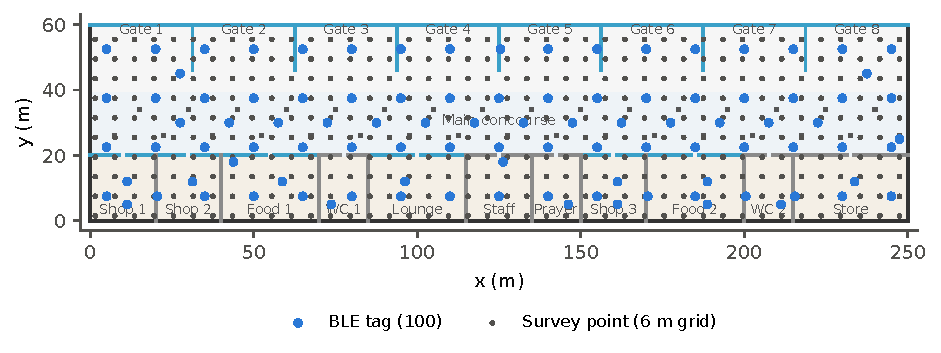
\includegraphics[width=\linewidth]{figures/floorplan.pdf}
  \caption{Simulated terminal: rooms (south), concourse with pillars (middle) and gates
  (north). Dark lines are concrete, grey drywall, blue glass. Dots are the 100 BLE tags;
  small grey points show the survey grid at \SI{6}{m} spacing.}
  \label{fig:floorplan}
\end{figure}

\subsection{Radio propagation with ray tracing}
The mean received power of every tag is computed with the Sionna~RT ray tracer at
\SI{2.426}{GHz} on a \SI{0.5}{m} grid at phone height (\SI{1.2}{m}), launching
$2\times10^8$ rays per tag with up to 8 interactions (reflection and transmission).
Walls use ITU material models (concrete \SI{20}{cm}, plasterboard \SI{10}{cm}, glass
\SI{2}{cm}). This gives realistic effects that simple formulas miss: reflections in the
tall hall, signal leaking through doorways, and stronger loss through ceilings.

\subsection{Phone measurements}
At each one-second scan the RSSI the phone reports for tag $i$ is
\begin{equation}
  z_i = \underbrace{P_i(\mathbf{p})}_{\text{ray tracing}}
      + \underbrace{s_i(\mathbf{p})}_{\text{shadowing}}
      - \underbrace{L^{\text{body}}_i - L^{\text{crowd}}_i - L^{\text{fade}}_i}_{\text{blocking}}
      + \underbrace{g_i}_{\text{Rician}}
      + \underbrace{b}_{\text{phone offset}}
      + \underbrace{e_i}_{\text{noise}},
  \label{eq:simulator}
\end{equation}
where $s_i$ is spatially correlated shadowing fixed to the building
($\sigma=\SI{3}{dB}$, correlation \SI{3}{m}); $L^{\text{body}}$ is up to \SI{10}{dB} when
the tag is behind the person; $L^{\text{crowd}}$ is \SI{5}{dB} per person on the line of
sight (capped at \SI{15}{dB}); $L^{\text{fade}}$ is a 10--\SI{20}{dB} deep fade with
probability 3\%; $g_i$ is Rician fading with $K=\SI{6}{dB}$; $b\sim\mathcal{N}(0,2^2)$ dB
is a constant offset of the phone for the whole walk; and $e_i\sim\mathcal{N}(0,1.5^2)$
dB. A reading is reported only if it exceeds the \SI{-95}{dBm} sensitivity and the packet
is received (probability 0.85). A phone typically hears 36--60 tags per scan, fewer in a crowd.

\subsection{Walks, crowds and steps}
Each test walk lasts \SI{600}{s}. The person walks along shortest paths between random
rooms, gates and concourse points at about \SI{1.3}{m/s} and pauses for 5--\SI{40}{s} at
half of them. The crowd consists of 0, 300, 800 or 2000 and other people walking the same way
(none, low, medium, high). The phone's step detector reports each step's length (true
stride about \SI{0.7}{m} with \SI{0.1}{m} noise) and heading change (\ang{1} noise plus a
gyro drift of about \SI{0.002}{rad/s}); 2\% of steps are missed.


%=====================================================================================
\section{Methodology}
\label{sec:method}
%=====================================================================================

\subsection{State}
Each particle $k$ carries the state
\begin{equation}
  \mathbf{x}^{(k)} = \bigl[\,x,\; y,\; \theta,\; \omega_b,\; \lambda\,\bigr]^{\top},
\end{equation}
the position in metres, the heading, the gyro bias (rad/s) and a stride scale factor.
The last two are constant per walk but unknown; carrying them in the state lets the
filter learn them, because particles with the wrong bias or stride drift away from the
measurements and are removed by resampling.

\subsection{Motion model}
The filter is driven by detected steps rather than by time. For a step of measured
length $\ell$ and heading change $\Delta\theta$, detected $\Delta t$ seconds after the
previous one, every particle is propagated as
\begin{align}
  \theta  &\leftarrow \theta + \Delta\theta - \omega_b\,\Delta t + \varepsilon_\theta,
           & \varepsilon_\theta &\sim \mathcal{N}(0,\, (\ang{3})^2), \label{eq:motion-heading}\\
  d       &= \lambda\,\ell + \varepsilon_d, & \varepsilon_d &\sim \mathcal{N}(0,\, 0.08^2\,\text{m}^2),\\
  \begin{bmatrix} x \\ y \end{bmatrix} &\leftarrow
  \begin{bmatrix} x \\ y \end{bmatrix} + d\begin{bmatrix} \cos\theta \\ \sin\theta \end{bmatrix}.
  \label{eq:motion-position}
\end{align}
At start-up $\omega_b\sim\mathcal{N}(0, 0.003^2)$ and $\lambda\sim\mathcal{N}(1, 0.1^2)$.
The heading noise is larger than the true per-step noise so that the particle cloud also
covers modelling errors such as turns that are not perfectly measured.

\paragraph{Map constraint.} If the straight move from the old to the new position
(checked at its end and its mid-point on a \SI{0.5}{m} occupancy grid) enters a wall,
pillar or outside the building, the particle's weight is set to zero. This is the
particle-filter equivalent of a likelihood $p(\text{map}\mid\mathbf{x}_{t-1},\mathbf{x}_t)$
that is 1 for feasible moves and 0 otherwise.

\subsection{Measurement models}

\label{sec:models}
Each scan gives RSSI readings $z_i$ for the tags that were heard. The measurement model
is $z_i = h_i(\mathbf{p}) + v_i$, where $\mathbf{p}=(x,y)$ and $h_i$ is the expected RSSI
of tag $i$ at that position. In words, $h_i$ answers one question for every particle:
\emph{if the phone really were here, what would it hear from tag $i$?} The filter then
compares that prediction with what the phone actually heard. Particles whose predictions
match the scan gain weight; particles whose predictions disagree lose it.

How well this works depends on how good the prediction is. Three choices of $h_i$ are
compared, each knowing more about the building than the last. Model~1 knows only the
distance to each tag. Model~2 also knows where the walls are. Model~3 knows what was
actually measured at each place. All three are fitted to or built from the same site
survey, so the comparison isolates the effect of the model itself. More knowledge gives
sharper predictions, but it also costs more to set up and maintain.

\paragraph{Model 1: plain log-distance path loss.}
\begin{equation}[H]
  h_i(\mathbf{p}) = A - 10\,n\,\log_{10} d_i(\mathbf{p}),
  \qquad d_i = \sqrt{(x-x_i)^2+(y-y_i)^2+(z_i-1.2)^2},
  \label{eq:plain}
\end{equation} .

A radio signal spreads out as it travels, so the power arriving at the phone
falls the further away the tag is. Because the power spreads over an ever larger area,
it falls with the \emph{logarithm} of distance, so every doubling of distance costs the same
number of decibels. The model has only two numbers for the whole building. $A$ is the
RSSI expected \SI{1}{m} from a tag. $n$ is the path-loss exponent and says how fast the signal fades. In free space $n=2$, so each doubling of distance costs \SI{6}{dB}. The distance $d_i$ is measured in 3-D,
from the phone held at \SI{1.2}{m} to the tag on the ceiling.

A least-squares fit to the survey gives $A=\SI{-61.7}{dBm}$ and $n=1.31$, so here each
doubling of distance costs only $10 \times 1.31 \times \log_{10}2 \approx \SI{3.9}{dB}$.
The exponent is well below 2 because the hall acts partly like a waveguide.
Reflections from the floor, roof and walls keep distant signals stronger than in open
space.

The logarithm has an important consequence for localisation. The change in RSSI per
metre of movement is $10n/(d \ln 10) \approx 5.7/d$~dB/m. A tag \SI{2}{m} away changes by
about \SI{2.8}{dB} for every metre the phone moves, but a tag \SI{20}{m} away changes by
only \SI{0.3}{dB}, far below the \SI{6}{dB} measurement noise. Nearby tags therefore
carry almost all the position information, which is why the filter uses the strongest
tags in each scan (\cref{sec:likelihood}).

The model treats the building as empty and lines of equal expected RSSI are circles around
each tag, whatever lies in between. This makes it cheap (two numbers for the whole
building), but it is wrong wherever walls block the signal. A tag behind a wall reads
weaker than the model expects, so the model believes it is further away, and the
particles are pulled in the wrong direction.

\paragraph{Model 2: multi-wall (Motley--Keenan).}
\begin{equation}
  h_i(\mathbf{p}) = A - 10\,n\,\log_{10} d_i(\mathbf{p}) - \sum_{t} N_{i,t}(\mathbf{p})\,L_t,
  \label{eq:multiwall}
\end{equation}

In this equation $N_{i,t}(\mathbf{p})$ is the number of walls of type
$t\in\{\text{concrete},\text{drywall},\text{glass},\text{ceiling}\}$ crossed by the
straight line from the phone to the tag, found by intersecting that 3-D line with every
wall segment of the floor plan, and $L_t$ is the loss per wall.

This keeps Model~1 and fixes its main error. Every wall between the phone and
the tag absorbs part of the signal, so the model subtracts a fixed toll for each wall
the direct line crosses, with a different toll for each material. The floor plan is
already known to the filter, so this extra knowledge costs nothing to collect. The equal-RSSI lines are no longer circles and they step down
wherever they cross a wall. The ceiling term covers the hall tags at \SI{10}{m}, which a
phone inside a room hears through the room's \SI{3}{m} ceiling.

The practical gain is at room boundaries. A tag inside a shop reads a few decibels
weaker from the concourse than from inside the shop, even at the same distance. The
plain model cannot see this difference, but the multi-wall model can, so it can better
tell whether the person has walked into the shop or is just passing its front.

A non-negative least-squares fit gives $A=\SI{-60.5}{dBm}$, $n=1.27$,
$L_\text{drywall}=\SI{1.5}{dB}$, $L_\text{glass}=\SI{1.7}{dB}$ and
$L_\text{ceiling}=\SI{4.4}{dB}$ (no surveyed reading crossed a concrete wall, so its
loss is undetermined). The wall losses are small at \SI{2.4}{GHz}, and signals also
reach the phone by reflection around the walls, which the model still ignores; so the
improvement over Model~1 is real but modest. To avoid tracing lines at run time,
$\sum_t N_{i,t}L_t$ is computed in advance for every tag on a \SI{1}{m} grid.

\paragraph{Model 3: fingerprint map.}
\begin{equation}
  h_i(\mathbf{p}) = M_i(\mathbf{p}),
  \label{eq:fingerprint}
\end{equation}
where $M_i$ is the surveyed mean RSSI of tag $i$ on a regular grid of spacing $\Delta$,
read between grid points by bilinear interpolation. Readings below the sensitivity are
stored as \SI{-95}{dBm}.

Instead of predicting the signal from physics, measure it. Before
deployment an installer walks the empty building and records the average RSSI of every
tag at each point of a grid. Each place then has its own pattern of strengths, for
example ``tag 12 strong, tag 40 medium, tag 7 weak'', much as a fingerprint identifies a
person. The map contains everything the formulas leave out like reflections, the
waveguide effect of the hall, shadows of pillars and the real losses of every wall. The
filter no longer needs an equation for the signal and for each particle it simply looks up
what the survey measured there.

A particle rarely sits exactly on a survey point, so the value is blended from the four
surrounding points, each weighted by how close the particle is to it (bilinear
interpolation). With $\Delta=\SI{3}{m}$, a particle at fractional grid offsets
$(u,v)\in[0,1)^2$ inside a cell with corner values $M_{00},M_{10},M_{01},M_{11}$ gets
\begin{equation}
  M_i(\mathbf{p}) = (1-u)(1-v)M_{00} + u(1-v)M_{10} + (1-u)v\,M_{01} + uv\,M_{11}.
\end{equation}
A particle exactly on a survey point gets that point's value, and one in the middle of a
cell gets the average of the four corners. The predicted field is therefore smooth and
continuous, which keeps nearby particles' weights similar.

The cost is effort and upkeep. The spacing sets the survey work: \SI{3}{m} needs 1660
points, \SI{6}{m} needs 420 and \SI{12}{m} needs 105. The \SI{6}{m} and \SI{12}{m} maps
keep every second or fourth point of the \SI{3}{m} survey. A coarser grid is cheaper but
blurs the map, because the interpolation has to bridge larger gaps, sometimes across a
wall. The map also describes the building on the day of the survey; if shops are refitted
or a beacon is moved, it goes out of date (\cref{sec:discussion}). \Cref{tab:models} summarises the three models.

\begin{table}[htbp]
  \centering
  \caption{What each measurement model knows, and what it costs.}
  \label{tab:models}
  \small
  \begin{tabular}{@{}p{0.2\linewidth}p{0.22\linewidth}p{0.25\linewidth}p{0.25\linewidth}@{}}
    \toprule
    Model & Knows about & Parameters & Set-up cost \\
    \midrule
    1. Plain path loss & distance only & $A$, $n$ & small survey to fit 2 numbers \\
    2. Multi-wall & distance and walls & $A$, $n$, one loss per wall type & floor plan and a small survey \\
    3. Fingerprint & measured signal at each place & one map value per tag and grid point & full grid survey, kept up to date \\
    \bottomrule
  \end{tabular}
\end{table}

\subsection{Likelihood and the phone offset}
\label{sec:likelihood}
Only the $K=10$ strongest readings of each scan are used. Weak readings are close to the
sensitivity limit, so they are biased (only lucky ones are heard) and add little
information. For particle $k$ let the residuals be
$r_i^{(k)} = z_i - h_i(\mathbf{p}^{(k)})$.

The phone offset $b$ in \cref{eq:simulator} shifts \emph{every} reading by the same
unknown amount. If it is ignored, a phone that reads \SI{6}{dB} low makes the true
position look poor, and the filter moves the person away from the tags. Treat the
residuals as $r_i = b + v_i$ with $v_i\sim\mathcal{N}(0,\sigma^2)$ and a prior
$b\sim\mathcal{N}(0,\tau^2)$. The posterior mean of $b$ given the $K$ residuals is
\begin{equation}
  \hat b = \frac{K\tau^2}{K\tau^2+\sigma^2}\;\bar r = \beta\,\bar r,
  \qquad \bar r = \frac1K\sum_{i=1}^K r_i ,
  \label{eq:offset}
\end{equation}
a shrinkage of the mean residual towards zero. The filter uses $\beta=0.5$, which
corresponds to $\tau^2=\sigma^2/K$, i.e.\ a prior offset spread of about \SI{1.9}{dB}
for $\sigma=\SI{6}{dB}$; this is close to the \SI{2}{dB} device offset of the simulator.
Removing only part of $\bar r$ keeps information about the absolute signal level, which
also depends on distance. In addition $\bar r$ is clipped to $\pm\SI{8}{dB}$ before
shrinking, so a particle in the wrong place (residuals of 10--\SI{20}{dB}) cannot explain
its error away as an offset. The log-likelihood of particle $k$ is then
\begin{equation}
  \log p\bigl(\mathbf{z}\mid\mathbf{x}^{(k)}\bigr) =
  \sum_{i=1}^{K} \log \mathcal{N}\!\Bigl(r_i^{(k)} - \beta\,\mathrm{clip}\bigl(\bar r^{(k)}, \pm 8\bigr);\; 0,\, \sigma^2\Bigr),
  \qquad \sigma = \SI{6}{dB}.
  \label{eq:likelihood}
\end{equation}

\subsection{Weight update, resampling and estimate}
Weights are updated as $w^{(k)} \leftarrow w^{(k)}\,p(\mathbf{z}\mid\mathbf{x}^{(k)})$
and normalised; the computation is done in log space, subtracting the largest
log-likelihood before exponentiating to avoid underflow. When the effective sample size
\begin{equation}
  N_\text{eff} = \Bigl(\sum_k \bigl(w^{(k)}\bigr)^2\Bigr)^{-1}
\end{equation}
falls below $N/2$, the particles are resampled with systematic resampling, which has
lower variance than multinomial resampling and costs $\mathcal{O}(N)$. Copied particles
are then moved by a small random jitter ($\sigma=\SI{0.15}{m}$, roughening) so that they
do not collapse onto one point, and 1\% of particles are re-drawn near the three
strongest tags of the current scan ($\sigma=\SI{6}{m}$). These injected particles let the
filter recover if it ever locks onto the wrong place. The reported position is the
weighted mean of the particles, and the heading is the weighted circular mean. \Cref{alg:pf} summarises one cycle.

\begin{algorithm}[H]
  \caption{One cycle of the BLE particle filter (one scan per second)}
  \label{alg:pf}
  \KwIn{particles $\{\mathbf{x}^{(k)}, w^{(k)}\}_{k=1}^N$, steps since the last scan, scan $\mathbf{z}$}
  \ForEach{detected step $(\ell, \Delta\theta, \Delta t)$}{
    propagate every particle with \cref{eq:motion-heading}--\cref{eq:motion-position}\;
    set $w^{(k)}=0$ for particles whose move crosses a wall\;
  }
  $\mathcal{S} \leftarrow$ the $K$ strongest tags in $\mathbf{z}$\;
  \For{$k=1$ \KwTo $N$}{
    $r_i^{(k)} \leftarrow z_i - h_i(\mathbf{p}^{(k)})$ for $i\in\mathcal{S}$ \tcp*{plain, multi-wall or map}
    $w^{(k)} \leftarrow w^{(k)}\,p(\mathbf{z}\mid\mathbf{x}^{(k)})$ using \cref{eq:likelihood}\;
  }
  normalise the weights\;
  \If{$N_\text{eff} < N/2$}{
    systematic resampling; roughen copies; re-draw 1\% near the strongest tags\;
  }
  \KwOut{$\hat{\mathbf{p}} = \sum_k w^{(k)}\mathbf{p}^{(k)}$, circular mean heading}
\end{algorithm}

%=====================================================================================
\section{Implementation}
\label{sec:implementation}
%=====================================================================================

The filter is written in Python with NumPy, vectorised over particles, so one cycle is a
handful of array operations rather than a loop over 3000 particles. The code is split so
that the three filters share everything except the measurement model.

\begin{center}
\small
\begin{tabular}{@{}ll@{}}
\toprule
File & Contents \\
\midrule
\texttt{filters/common.py} & settings, motion model, wall constraint, likelihood, resampling, run loop\\
\texttt{filters/plain.py} & Model 1, \cref{eq:plain}\\
\texttt{filters/multi\_wall.py} & Model 2, \cref{eq:multiwall}\\
\texttt{filters/fingerprint.py} & Model 3, \cref{eq:fingerprint}, with the map spacing as a setting\\
\bottomrule
\end{tabular}
\end{center}

\paragraph{Motion model.} One call moves all particles by one step and removes those that
hit a wall:
\begin{lstlisting}
def predict_step(self, length, turn, elapsed):
    c, n = self.config, len(self.xy)
    self.heading = self.heading + turn - self.bias * elapsed + self.rng.normal(0, c.heading_noise_rad, n)
    stride = self.scale * length + self.rng.normal(0, c.step_noise_m, n)
    move = np.column_stack([stride * np.cos(self.heading), stride * np.sin(self.heading)])
    target = self.xy + move
    blocked = ~(self.is_free(target) & self.is_free(self.xy + move / 2))
    target[blocked] = self.xy[blocked]
    self.weights[blocked] = 0.0
    self._normalise()
    self.xy = target
\end{lstlisting}

\paragraph{Likelihood and weight update.} The residual matrix has one row per particle
and one column per chosen tag; the offset of \cref{eq:offset} is removed per row:
\begin{lstlisting}
def log_likelihood(self, residual):
    c = self.config
    offset = np.clip(residual.mean(axis=1, keepdims=True), -c.offset_limit_db, c.offset_limit_db)
    return gaussian_logpdf(residual - c.offset_shrink * offset, c.ble_sigma_db).sum(axis=1)

def update(self, rssi):
    tags = self.strongest(rssi, self.config.ble_top_k)
    if len(tags) == 0:
        return
    log_like = self.log_likelihood(rssi[tags] - self.expected_rssi(tags))
    alive = self.weights > 0
    peak = log_like[alive].max() if alive.any() else log_like.max()
    self.weights = self.weights * np.exp(np.clip(log_like - peak, -300, 0))
    self._normalise()
\end{lstlisting}

\paragraph{The three measurement models.} Each filter only defines
\texttt{expected\_rssi}, which returns an array of shape (particles, tags):
\begin{lstlisting}
class PlainFilter(ParticleFilter):                      # Model 1
    def expected_rssi(self, tags):
        return self.a_dbm - 10 * self.n * np.log10(tag_distance(self.xy, self.tags[tags]))

class MultiWallFilter(ParticleFilter):                  # Model 2
    def expected_rssi(self, tags):
        free_space = self.a_dbm - 10 * self.n * np.log10(tag_distance(self.xy, self.tags[tags]))
        return free_space - self.wall_loss(tags)        # precomputed sum of N_t * L_t

class FingerprintFilter(ParticleFilter):                # Model 3
    def expected_rssi(self, tags):
        coords = (self.xy[:, ::-1].T - self.origin) / self.map_spacing_m
        return np.stack([map_coordinates(self.ble_map[t], coords, order=1, mode="nearest")
                         for t in tags], axis=1)
\end{lstlisting}

\paragraph{Resampling.} Systematic resampling draws one uniform number and places $N$
evenly spaced pointers on the cumulative weights:
\begin{lstlisting}
def systematic_resample(weights, rng):
    positions = (rng.random() + np.arange(len(weights))) / len(weights)
    return np.searchsorted(np.cumsum(weights), positions).clip(0, len(weights) - 1)
\end{lstlisting}

\paragraph{Testing.} Unit tests check each building block: the Gaussian density, that
resampling follows the weights, that the offset removal is partial and capped as in
\cref{eq:offset}, that particles cannot cross a wall, each measurement model against a
hand-computed value (including bilinear interpolation between survey points), and that
the filter tracks a simple straight walk.

%=====================================================================================
\section{Experimental Setup}
\label{sec:setup}
%=====================================================================================

All results in this report use 10 walks (random seeds 90--99) that were not used while
developing the filter, each simulated at all four crowd levels, so every method is
scored on the same 40 walks of \SI{600}{s}. Errors are measured once per second against
the true position after a \SI{30}{s} settling period. The metrics are:
\begin{itemize}
  \item \textbf{Median and 90th-percentile position error} over all scans of all walks,
        and the root-mean-square error (RMSE), which is sensitive to large failures;
  \item \textbf{heading error}, the median absolute difference to the true walking direction;
  \item \textbf{correct room} (share of time inside a room that the estimate is in the
        same room) and \textbf{correct hall} (share of time in the hall that the estimate
        is in the hall);
  \item \textbf{run time} per scan on one laptop CPU core with 3000 particles.
\end{itemize}
When two methods are compared, the per-walk median errors are paired by walk, and a
bootstrap over walks gives a 95\% interval for the mean difference. Two simple
baselines show what the filter adds:
\textbf{BLE centroid}, the RSSI-weighted average position of the four strongest tags
in each scan with no filtering; and \textbf{steps only}, dead reckoning from the true
starting position and heading with no radio at all.

%=====================================================================================
\section{Results}
\label{sec:results}
%=====================================================================================

\subsection{How the filter works on one walk}
\Cref{fig:particles} shows the particle cloud on one walk with a medium crowd. At the
first scan the particles are spread around the three strongest tags, about
\SI{20}{m} across, and the estimate is several metres off. After a few seconds of steps
and scans the wrong hypotheses have been removed, and by \SI{30}{s} the cloud is a few
metres wide around the true position. \Cref{fig:trajectories} shows the whole
\SI{10}{min} walk for the three measurement models, and \cref{fig:error-time} shows the
error over time. The fingerprint filter follows the path closely, including the room
visits on the right; the two formula-based filters drift up to \SI{10}{m}, mostly in the
last third of the walk where the person stays in the gate area.

\begin{figure}[htbp]
  \centering
  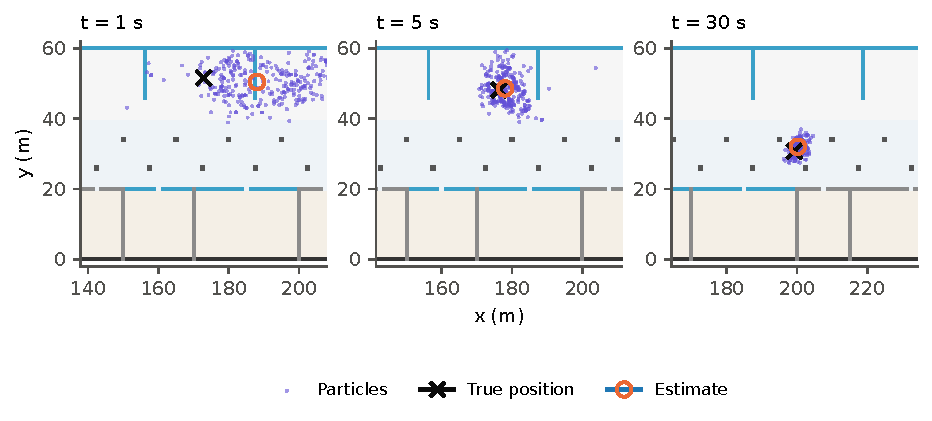
\includegraphics[width=\linewidth]{figures/particles.pdf}
  \caption{Particle cloud of the \SI{6}{m} fingerprint filter (300 of 3000 particles
  shown) at 1, 5 and \SI{30}{s} into a walk with a medium crowd. The cloud starts
  around the strongest tags and contracts onto the true position.}
  \label{fig:particles}
\end{figure}

\begin{figure}[htbp]
  \centering
  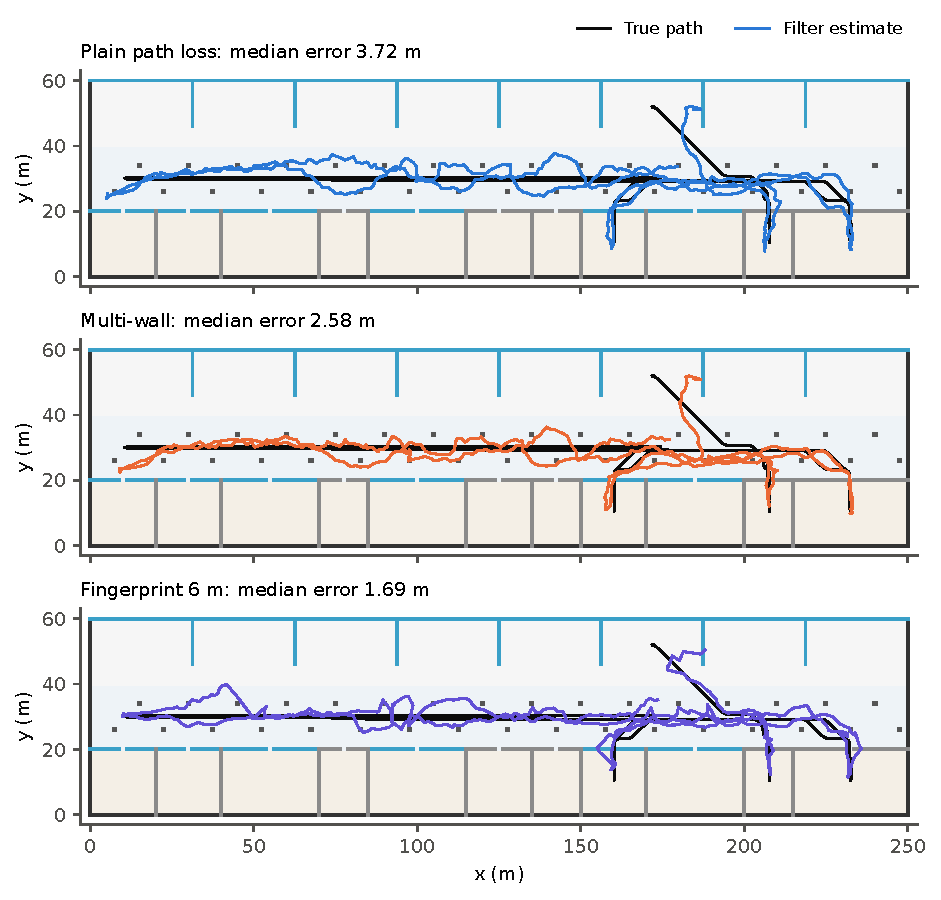
\includegraphics[width=\linewidth]{figures/trajectories.pdf}
  \caption{True path (black) and filter estimate for one \SI{10}{min} walk with a medium
  crowd, for the three measurement models.}
  \label{fig:trajectories}
\end{figure}

\begin{figure}[htbp]
  \centering
  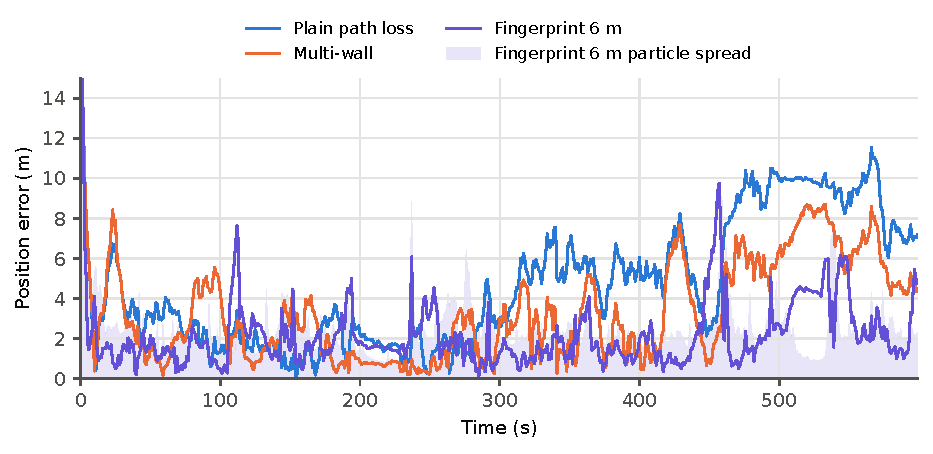
\includegraphics[width=\linewidth]{figures/error_time.pdf}
  \caption{Position error over time for the walk of \cref{fig:trajectories}. The shaded
  band is the spread (RMS distance of particles from the estimate) of the
  \SI{6}{m} fingerprint filter, the filter's own estimate of its uncertainty.}
  \label{fig:error-time}
\end{figure}

\paragraph{3D visualisation.} To show the filter running in the terminal, one walk was also
rendered in NVIDIA Isaac Sim (\cref{fig:isaac}). It is a separate walk from the one
above: no crowd in the radio simulation, the first \SI{82}{s} of the walk, replayed through
the \SI{6}{m} fingerprint filter, with a median error of \SI{1.45}{m} over that stretch.
Every moving part of the render comes from the filter run: the person follows the true
path from the simulation log, the orange particles are 320 of the filter's 3000, and the
cyan ring and trail are the weighted-mean estimate. The beacons drawn lit are the ten
strongest in the latest scan, which the filter uses. A few things were changed for the
picture only: walls and pillars are cut to \SI{3}{m} and the roof is left off so the camera
can see in, the concourse beacons are drawn at \SI{4}{m} instead of \SI{10}{m}, and the
other people are animated figures that do not affect the radio signal. A top-down
Matplotlib animation of the same walk accompanies the 3D video.

\begin{figure}[htbp]
  \centering
  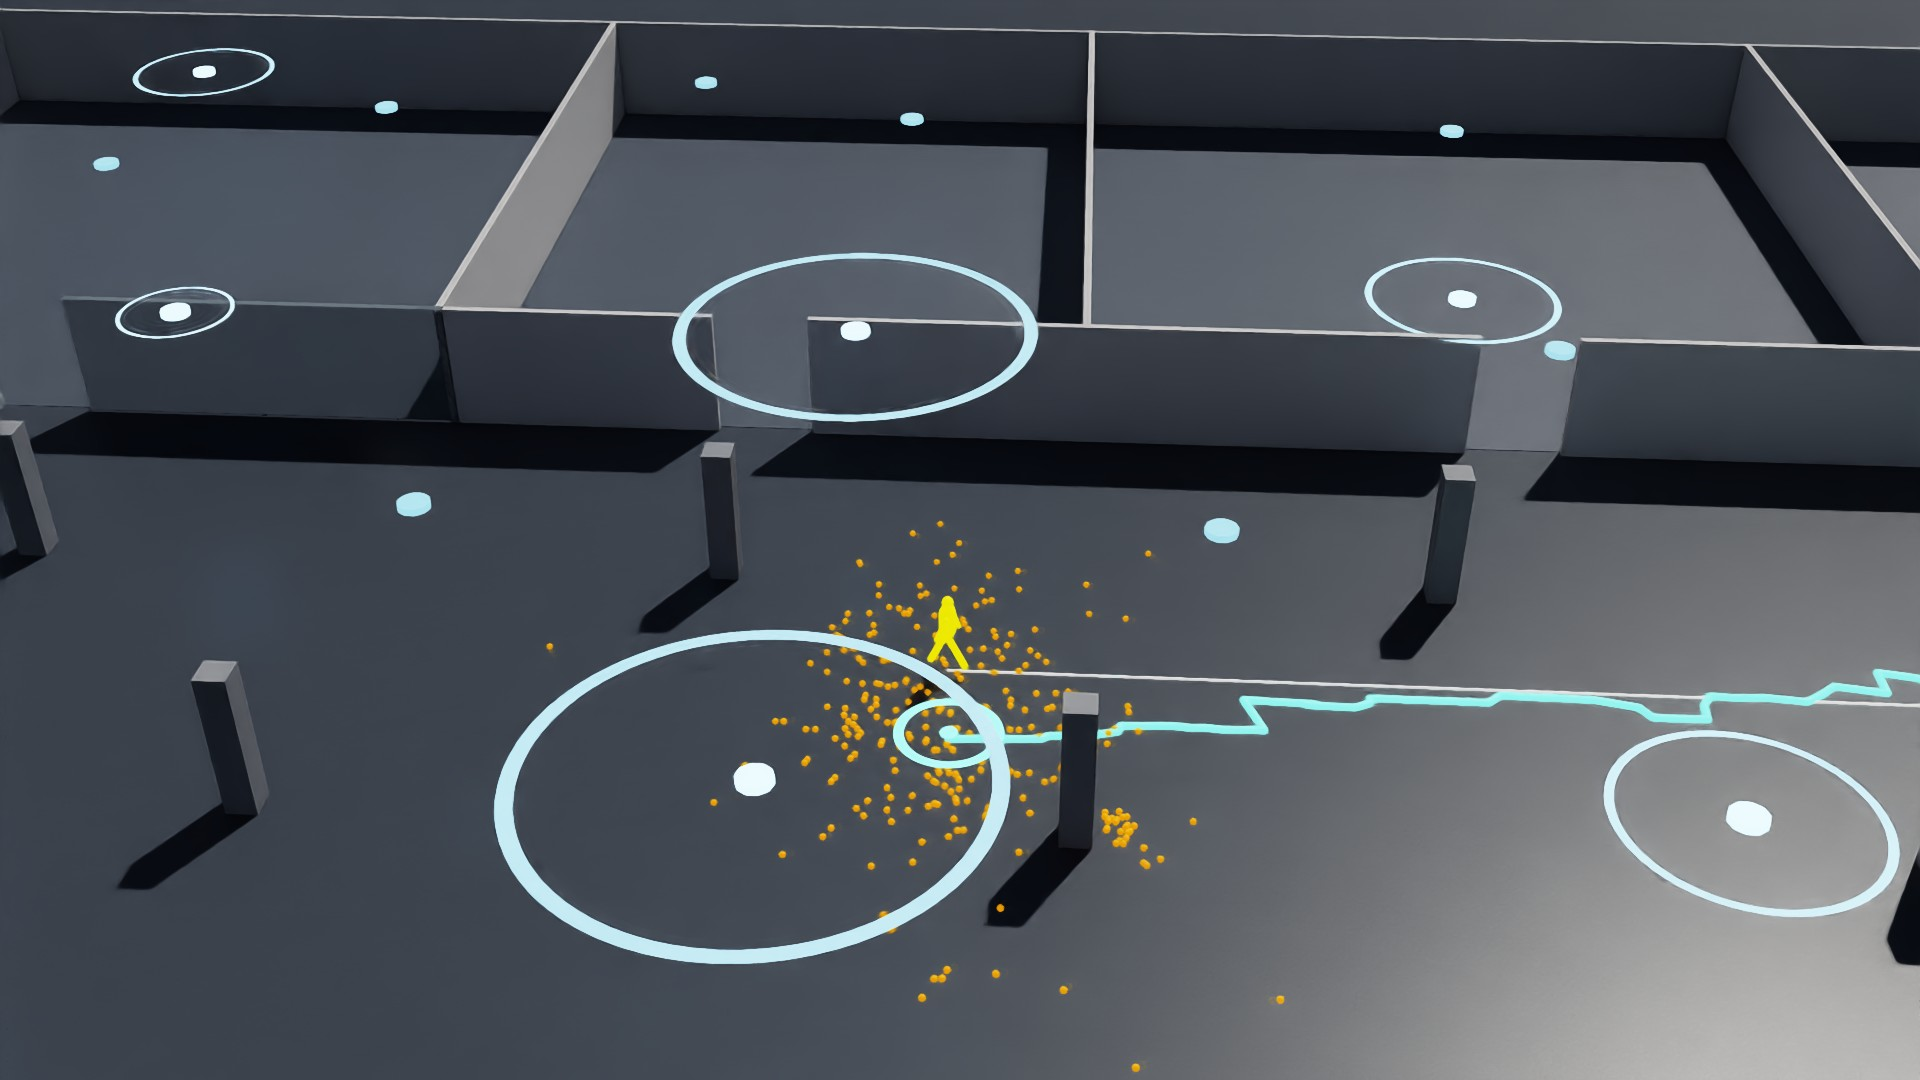
\includegraphics[width=\linewidth]{figures/isaac_render.jpg}
  \caption{Isaac Sim render of the \SI{6}{m} fingerprint filter tracking a walker (yellow)
  along the concourse, \SI{42}{s} into the walk. Orange: particles; cyan ring and line:
  estimate and estimated path; thin white line: true path; blue discs with rings: BLE
  beacons used in the current scan. The estimate is \SI{2.2}{m} from the person in this
  frame.}
  \label{fig:isaac}
\end{figure}

\subsection{Comparison of the measurement models}
\Cref{tab:main} and \cref{fig:cdf} summarise all 40 walks.

\begin{table}[htbp]
  \centering
  \caption{Results over 40 walks (10 walks $\times$ 4 crowd levels). Errors are in
  metres. Heading is meaningless for the BLE centroid, which has no motion model.}
  \label{tab:main}
  \small
  \begin{tabular}{@{}lrrrrrrrr@{}}
    \toprule
    Method & Median & p90 & RMSE & $<\SI{2}{m}$ & Heading & Room & Hall & ms/scan\\
    \midrule
    Plain path loss      & 3.45 & 7.64 & 4.76 & 27\% & \ang{6.8} & 96.2\% & 98.6\% & 6.6\\
    Multi-wall           & 3.13 & 7.17 & 4.48 & 31\% & \ang{6.7} & 95.1\% & 99.7\% & 6.8\\
    Fingerprint \SI{3}{m}  & \textbf{1.30} & \textbf{2.83} & \textbf{2.15} & \textbf{76\%} & \textbf{\ang{5.0}} & 95.1\% & 99.9\% & 7.8\\
    Fingerprint \SI{6}{m}  & 1.70 & 3.66 & 2.50 & 61\% & \ang{5.3} & 87.4\% & 100.0\% & 7.8\\
    Fingerprint \SI{12}{m} & 2.44 & 5.72 & 3.73 & 38\% & \ang{6.4} & 90.7\% & 99.8\% & 7.8\\
    \midrule
    BLE centroid (no filter) & 8.40 & 17.23 & 11.38 & 5\% & -- & 83.9\% & 92.1\% & $<0.1$\\
    Steps only (no radio)    & 24.56 & 96.00 & 65.66 & 4\% & \ang{40.9} & 20.9\% & 71.0\% & $<0.1$\\
    \bottomrule
  \end{tabular}
\end{table}

\begin{figure}[htbp]
  \centering
  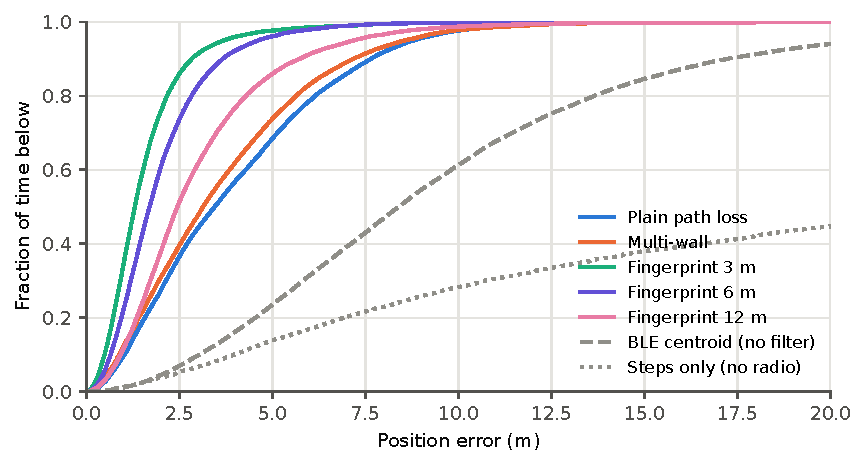
\includegraphics[width=0.85\linewidth]{figures/cdf.pdf}
  \caption{Cumulative distribution of position error over all 40 walks.}
  \label{fig:cdf}
\end{figure}

\paragraph{The filter itself matters most.} Every filter is far better than either
baseline. The BLE centroid has a median error of \SI{8.4}{m}: one scan alone is too noisy
and the strongest tags are often not the nearest. Steps alone drift by tens of metres
within minutes because small heading errors accumulate. Combining the two in the
particle filter with the floor plan reduces the median error by a factor of 2.5 to 6.5.

\paragraph{The measurement model is the second largest factor.} Adding walls to the
path-loss model helps a little ($-0.37$ m on average, 95\% interval $-0.66$ to
$-0.10$, better in 22 of 40 walks). The fingerprint map helps much more: the \SI{6}{m}
map is \SI{1.53}{m} better than multi-wall (interval $-1.91$ to $-1.17$, better in 38 of
40 walks). Survey density matters: each halving of the spacing reduces the median error,
from \SI{2.44}{m} at \SI{12}{m} to \SI{1.70}{m} at \SI{6}{m} and \SI{1.30}{m} at
\SI{3}{m} (6 m vs 12 m better in 37/40 walks; 3 m vs 6 m better in 36/40). Even the
coarse \SI{12}{m} map, which needs only 105 survey points, beats the multi-wall model by
\SI{0.77}{m} (better in 32/40).

\Cref{fig:model-maps} shows why. For a tag inside a room, the plain model predicts a
smooth circular pattern that ignores walls. The multi-wall model adds steps at walls but
uses one fitted loss per wall type. The surveyed map captures what really happens,
including reflections in the tall hall and the much weaker signal behind the room's
front wall and ceiling.

\begin{figure}[htbp]
  \centering
  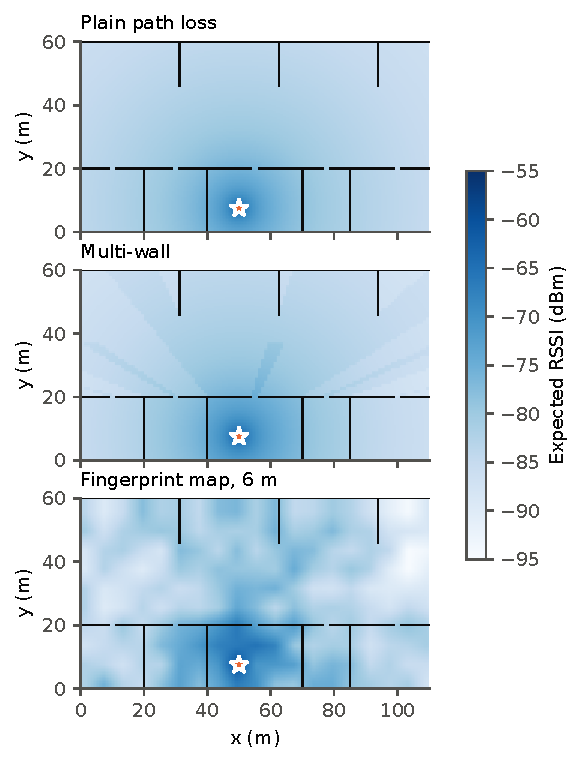
\includegraphics[width=0.8\linewidth]{figures/model_maps.pdf}
  \caption{Expected RSSI of one tag (star) inside a room under each measurement model,
  for the western part of the terminal.}
  \label{fig:model-maps}
\end{figure}

\paragraph{Correct room.} The \SI{6}{m} map identifies the right room only 87\% of the
time, less than both the coarser \SI{12}{m} map and the formula models, even though its
position error is smaller. A likely cause is the interpolation: on the \SI{6}{m} grid,
the survey points nearest to the room fronts ($y=\SI{20}{m}$) lie at
$y=\SI{19.5}{m}$ inside the rooms and $y=\SI{25.5}{m}$ in the hall, so the interpolated
map blends room and hall signal across the wall, and particles just outside a door look
as likely as those inside. The \SI{3}{m} map, with points \SI{1.5}{m} either side of the
wall, does not have this problem (95\%). This explanation was not tested separately.

\subsection{Effect of crowds}
\Cref{fig:crowd} shows the median error per crowd level. Crowds of up to 2000 people
increase the fingerprint filters' error by \SIrange{0.3}{0.6}{m} (high crowd vs no crowd
on the same walks: $+0.30$, $+0.46$ and $+0.59$ m for the 3, 6 and \SI{12}{m} maps, worse
in 8--9 of 10 walks). The two formula filters show no consistent crowd effect: their
error is dominated by model error, not by the extra blocking. All filters remain far
better than the baselines at every crowd level.

\begin{figure}[htbp]
  \centering
  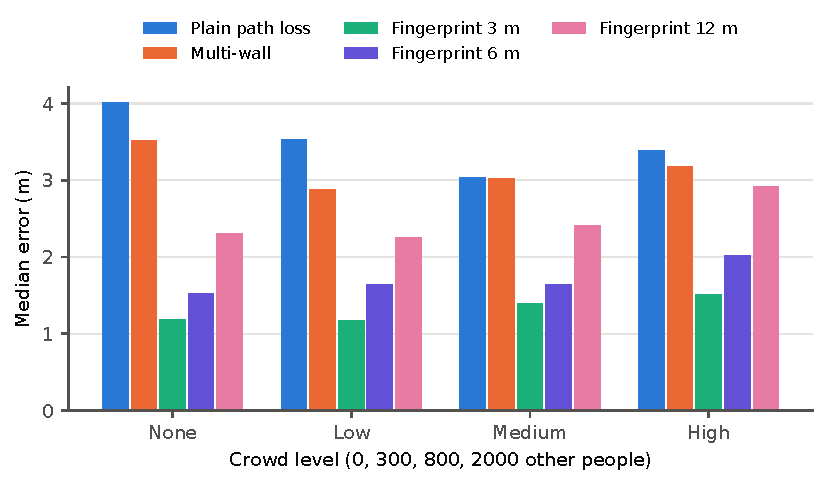
\includegraphics[width=0.85\linewidth]{figures/crowd.pdf}
  \caption{Median position error by crowd level for the five filters.}
  \label{fig:crowd}
\end{figure}

\subsection{Parameter study}
\label{sec:sweeps}
The \SI{6}{m} fingerprint filter was re-run while changing one parameter at a time, on the
same 10 walks with no crowd and with a high crowd (\cref{fig:sweeps}). The plotted value
is the mean of the 10 per-walk median errors, together with the worst walk.

\begin{figure}[htbp]
  \centering
  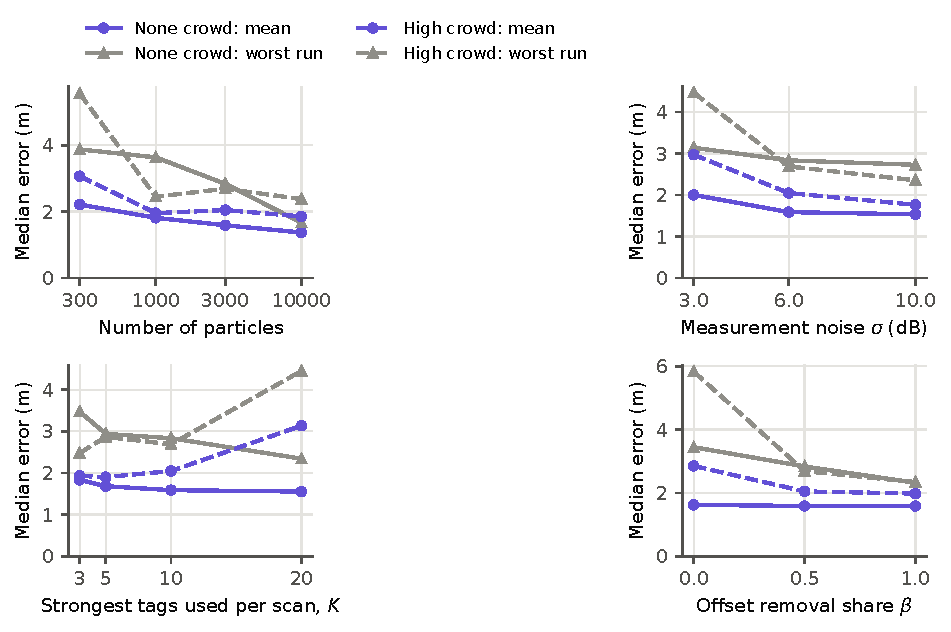
\includegraphics[width=0.9\linewidth]{figures/sweeps.pdf}
  \caption{Sensitivity of the \SI{6}{m} fingerprint filter to one parameter at a time.
  Purple: mean of per-walk median errors; grey: worst walk. Solid: no crowd; dashed:
  high crowd.}
  \label{fig:sweeps}
\end{figure}

\begin{itemize}
  \item \textbf{Number of particles.} Error falls from \SI{2.2}{m} with 300 particles to
        \SI{1.4}{m} with 10\,000 (no crowd), with diminishing returns beyond 3000. Run
        time grows roughly linearly, from \SI{1.8}{ms} to \SI{25}{ms} per scan. 3000
        particles is a reasonable balance: about \SI{8}{ms} per scan, so one core can
        track over 100 phones in real time at one scan per second.
  \item \textbf{Measurement noise $\sigma$.} Too small a value ($\sigma=\SI{3}{dB}$)
        makes the filter over-confident: weights collapse onto a few particles and the
        error rises to \SI{3.0}{m} in a crowd. A larger value is safer under crowds:
        $\sigma=\SI{10}{dB}$ gave \SI{1.76}{m} against \SI{2.05}{m} for the default
        \SI{6}{dB}, with almost no change without a crowd. Readings in one scan share
        errors (body and crowd blocking), so treating 10 readings as independent
        overstates the evidence; a larger $\sigma$ compensates for this.
  \item \textbf{Strongest tags used, $K$.} Without a crowd more tags help slightly. With a
        high crowd, $K=20$ is clearly worse (\SI{3.1}{m}): the extra tags are weaker, more
        often blocked, and close to the sensitivity limit, where only readings that
        happen to be strong are heard. $K$ between 3 and 10 gives similar results.
  \item \textbf{Offset removal $\beta$.} Without offset removal ($\beta=0$) the filter is
        fine with no crowd, but under a high crowd its error rises to \SI{2.85}{m}, its
        90th percentile to \SI{8.9}{m}, and one walk reached a median of \SI{5.8}{m}.
        Crowd blocking and the phone offset lower all readings together, and without
        the correction the filter explains this by moving the person away from the
        tags. Both $\beta=0.5$ and $\beta=1$ prevent this.
\end{itemize}
These sweeps use the same walks as \cref{tab:main}, so the defaults were fixed before these
walks were run, and they were not re-tuned on them.

%=====================================================================================
\section{Discussion}
\label{sec:discussion}
%=====================================================================================

\paragraph{Why a particle filter fits this problem -} Three parts of the design could
not be expressed in a Kalman filter. The map constraint removes particles that walk
through walls, which keeps the estimate inside corridors and rooms. The fingerprint
measurement model is a lookup table with no derivative. And at start-up, or after a
wrong turn, the cloud holds several hypotheses at once (\cref{fig:particles}). The
per-particle gyro bias and stride scale are a cheap way to estimate slowly varying
sensor errors: they need no extra equations, only resampling.

\paragraph{What limits accuracy -} The formula models are limited by model error, not
noise: a single path-loss exponent cannot describe both nearby tags and the reflections
that keep distant tags strong. In the survey data, tags within \SI{5}{m} read about
\SI{4}{dB} stronger than the fitted plain model predicts, while far tags match it, so the
filter is systematically pulled away from nearby tags. The fingerprint map removes this
bias, which is why it wins by a large margin. Its own limit is the survey spacing and the
interpolation between survey points.

\paragraph{Problems found and how they were addressed -} Several design choices came from
failures seen during development:
\begin{itemize}
  \item An early model subtracted a fixed loss for every tag in a different zone (room
        or hall). In the hall this pulled estimates several metres sideways towards the
        rooms, because the fixed loss was larger than the real loss through glass fronts.
        Replacing it with wall counts (Model 2), and then with a map (Model 3), removed
        the drift.
  \item Using every heard tag instead of the strongest 10 made the error much worse because
        weak readings are biased high because only lucky ones pass the sensitivity limit.
  \item Without offset removal, a phone that read about \SI{6}{dB} low in a crowd made
        the filter lose the person completely on one walk during development
        (median error \SI{34}{m}). The shrinkage estimate of \cref{eq:offset} fixed this,
        and the parameter study above confirms it.
  \item A heavy-tailed Student-$t$ likelihood was compared with the Gaussian on 40 walks and
        the two were tied for the fingerprint maps and the Gaussian was slightly better
        for the formula models, so the simpler Gaussian was kept.
  \item Choosing the strongest tags after adding back each particle's modelled wall
        loss (so a tag behind a wall is not unfairly dropped) changed only about one tag
        in ten and gave no measurable gain.
\end{itemize}

\paragraph{Map staleness -} A fingerprint map describes the building on the day of the
survey. To test what happens when the building changes, the \SI{6}{m} map was perturbed
by a smooth random error per tag plus a constant error per tag, while the phone readings
stayed the same (\cref{tab:stale}).

\begin{table}[h]
  \centering
  \caption{\SI{6}{m} fingerprint filter with an out-of-date map: mean of the 10 per-walk
  median errors (worst walk in brackets), in metres. For comparison, the multi-wall
  filter scores 3.69 (no crowd) and 3.39 (high crowd) on the same walks.}
  \label{tab:stale}
  \small
  \begin{tabular}{@{}lrr@{}}
    \toprule
    Map error added (smooth field + per tag) & No crowd & High crowd\\
    \midrule
    None                                 & 1.59 (2.83) & 2.05 (2.69)\\
    \SI{3}{dB} + \SI{1}{dB}             & 2.19 (3.53) & 2.62 (3.41)\\
    \SI{5}{dB} + \SI{2}{dB}             & 3.41 (5.69) & 4.88 (7.58)\\
    \SI{8}{dB} + \SI{3}{dB}             & 7.07 (10.37) & 7.56 (13.37)\\
    \bottomrule
  \end{tabular}
\end{table}

Small changes (about \SI{3}{dB}) cost about half a metre. Around \SI{5}{dB} the map is no
better than the multi-wall formula, and at \SI{8}{dB} it is much worse. A deployed system
therefore needs the map to be checked after changes to the building, or updated
automatically; the error sizes used here are assumptions, and real drift can only be
measured in a pilot.

\paragraph{Limitations -} All data is simulated. The ray tracer has no furniture, shop
fittings or people, and the same simulated building produced both the survey and the
test walks, so the fingerprint map here is close to perfect; real accuracy will be lower
and must be measured in a pilot. Only one demonstration building was simulated, so other layouts (for example a
multi-storey mall with an atrium) remain to be tested. Only one floor and one person are
tracked, the phone is
always held at \SI{1.2}{m}, and the step detector is simulated rather than real.

%=====================================================================================
\section{Conclusion}
\label{sec:conclusion}
%=====================================================================================

A particle filter was implemented for indoor localisation in large facilities such as
airports and shopping malls. It tracks a pedestrian by fusing BLE signal strength with
smartphone IMU step detection, with the floor plan as a hard constraint, and was
demonstrated in a simulated \SI{15000}{m^2} airport terminal. Using the same filter with three measurement models showed that the
model of the radio signal is decisive: a fingerprint map from a site survey reduced the
median error from \SI{3.1}{m} (multi-wall) to \SI{1.7}{m} at \SI{6}{m} survey spacing and
\SI{1.3}{m} at \SI{3}{m}, with 90\% of errors below \SI{2.8}{m} for the denser map.
The filter stays accurate with crowds of 2000 people, runs in about \SI{8}{ms} per scan
on one CPU core, and is 5--6 times more accurate than using BLE or steps alone.
Removing a shrunken estimate of the shared reading offset was essential for robustness
in crowds.

\paragraph{Future work -} Test on real phones in a real airport or shopping mall; use a wall-aware interpolation of
the map so that survey points on the other side of a wall are not blended in; adapt
$\sigma$ to the crowd level; and update the map over time from the filter's own
confident estimates to counter map staleness.

\end{document}
